\chapter{Topic Information and Speech Retrieval}
\label{sec:retrieval1}
\label{sec:repetitionRetrieval}
\label{sec:topicLMsRetrieval}

\chaptermark{Topic Information and Speech Retrieval}

Having considered the strength of the topic signal from the perspective of classification, we analyze the impact of topic information on the keyword retrieval task.  We shift our focus from a supervised setting, where the user information need is expressed explicitly by labeled examples, to an unsupervised setting, where queries are expressed as key words or phrases.  In this chapter we demonstrate how both \textit{local} context, in terms of repetition and cache-based language models, and \textit{broad} context, expressed as latent topic mixture models, individually and jointly, improve keyword retrieval performance.  The results in this chapter motivate the joint model of both contexts that follows in Chapter~\ref{sec:klda}.

To understand how word context can affect keyword performance, we describe standard approaches for generating keyword scores from ASR systems.  We are going to incorporate topical word contexts primarily by modifying the ASR system's language model.  Both interpolation-based approaches to adapting standard backoff N-gram language models and more recent discriminative language model re-scoring can be expressed expressed in terms of finite state transducer (FST) operations.  Through the FST formulations we present a contrastive view of the adaptation approaches before looking at the empirical performance.

We then present a keyword-specific method for leveraging local (within-document) repetition in any speech retrieval system.  By using only the KWS score, and treating the retrieval system as a black box, we can incorporate local context without modifying the underlying speech recognition models.  This approach, which we describe in Section~\ref{sec:repetitionModel}, is generally applicable to any KWS system and improves retrieval performance across a spectrum of language conditions.  However, this approach only incorporates the repetition aspect of topic context.

By contrast, in the latter part of this chapter, we show how we can apply both latent topics (broad context) and cached N-grams (local context) directly to the recognizer's language model.  By interpolating unigrams from broad topic context derived from a standard LDA topic model\cite{blei2003latent,steyvers2007} we improve retrieval performance by up to 1\% absolute via lattice re-scoring (applying a new N-gram language model to the recognition output).  Re-decoding with the same topic-adapted language model improves accuracy by up to 2.1\%.  Adding local context via cached N-grams improves performance by up to 1.6\%.  A cascaded approach - re-decoding with latent topics then re-scoring with cached N-grams - gives an overall absolute improvement of up to 2.4\%.  For all languages we consider, combining broad and local topic information into the language model outperforms each individual method.

\section{Lattice-based Keyword Scores}
\label{sec:scores}
In the previous chapter we briefly mentioned that when using ASR word outputs either for keyword search or classification, we typically use the posterior probability of a particular word output in computing expected counts for feature generation or for ranking keyword results.  In this section define how these scores are computed and formally illustrate how the ASR/KWS output is impacted by language model-based techniques for incorporating topic information.

We start with the definition of the posterior probability of a word hypothesis $w_i$ given the word lattice output $\mathcal{L}$ of an ASR system for a single segment of acoustic input.  The posterior and subsequently the ASR/KWS scores are composed using the various ASR model likelihoods for the word $w_i$ given the acoustic input: acoustic model $l_{AM}$, language model $l_{LM}$ and HMM transition model, $l_{H}$.  At this level modifications or adaptions of the language model occur.  

A speech recognition lattice $\mathcal{L}$ is a directed acyclic graph representing the ASR system's hypothesized set of word sequences $W=\{w_1,...,w_n\}$ for a fixed amount of acoustic input.  The nodes (states or vertices) of $\mathcal{L}$ correspond to particular locations in the input.  The arcs (or edges) are labeled with the words $w_i$ to be output for the corresponding input.  The model likelihoods for an arc $a$ with output label $w_i$ are captured in a weight or set of weights on $a$.  A subset of the nodes are marked initial nodes and a subset are denoted as final.  We denote a sequence of arcs staring at an initial state and ending with a final state as a path $\pi$.  We denote a path that passes through the arc $a$ with word hypothesis $w_0$ as $\pi[a]$.  With this instantiation we can safely treat $\mathcal{L}$ as a finite state transducer (cf. \cite{povey2012}).

The path likelihoods $l(\pi)$ are given by multiplying the acoustic, language, and transition model probabilities along the arcs in the path (Eqn.~\ref{pathLikelihood}).  We compute the posterior probability of a word hypothesis $p(w_0|a,\mathcal{L})$ as the fraction of the fraction of the total likelihood captured by the paths that contain the arc $a$ (Eqn.~\ref{arcPosterior}).
\begin{align}
%&\text{Path Likelihood} &
l(\pi) &= \prod_{a_i \in \pi} l_{AM}(a_i) \cdot l_{LM}(a_i) \cdot l_{H}(a_i) \label{pathLikelihood} \\[1ex]
%&\text{Posterior} & 
p(w_0|a,\mathcal{L}) &= \frac{\sum_{\pi_i[a] \in \mathcal{L}}l(\pi_i[a])}{\sum_{\pi \in \mathcal{L}} l(\pi)} \label{arcPosterior} \\[1ex]
%&\text{KWS Score} & 
S_{KWS}(h_{\mathcal{L},w_0,i}) &= \sum_{a \in A(w_0)} p(w_0|a,\mathcal{L}) \label{kwsScore}
\end{align} 
\vskip0.2cm

In practice $\mathcal{L}$ often contains multiple arcs with slightly different starting times for the same word.  This effectively dilutes the posterior probability for a single word occurrence across multiple arcs.  In KWS systems, arcs covering similar time intervals are clustered and the arc posteriors are summed to obtain a single posterior detection score $S(w_0)$ for $w_0$ (cf.~\cite{miller2007rapid}).  We distinguish the word type $w_0$ from the $i^{th}$ cluster of arcs $C_i(w_0)$, which corresponds to a single KWS system output hypothesis $h_{\mathcal{L},w_0,i}$.

Our first proposed method of keyword-based repetition re-scoring (Section~\ref{sec:repetitionModel}) operates directly on this KWS score. The rest of the methods discussed in this chapter impact the language model likelihood directly.  The LM probabilities contribute to the KWS score computation through the path likelihoods, composed of individual arc likelihoods.
% inference is done on the soft word counts which does contain acoustic information

In many current ASR implementations, output lattices are indeed instantiated as Weighted Finite State Transducers (WFSTs). Typically the above likelihoods are captured by the weights on the WFST transitions, interpreted as \textit{costs}, and stored as negative log-likelihoods.  Standard FST operations such as determinization and minimization (cf. \cite{mohri2002weighted}) can be applied and are typically done in negative log space.

The output lattice $\mathcal{L}$ can also be considered a realization of the composition of an FST consisting of the acoustic input (U) for each frame (discrete input time step, typically 100ms) and the decoding graph, denoted $HCLG$, which combines the lexicon (L), language model (G), context-dependencies (C) and HMM structure (H)\cite{povey2012}:
\begin{equation}
\mathcal{L} \approx S \equiv U \circ HCLG
\end{equation}
\noindent We conflate the definitions given in \cite{povey2012} to indicate that the actual lattice $\mathcal{L}$ is obtained by heuristically pruning the true search space $S$.  Additionally, the lattices generated in the Kaldi WFST implementation (following \cite{povey2012}) conflate the language model and transition model probabilities into a ``graph cost".  From this we can express the path cost as:
\begin{equation}
-\log(l(\pi)) = \sum_{a_i \in \pi} -\log(l_{AM}(a_i)) - \log(l_{LM}(a_i)) - \log(l_{H}(a_i))\label{lm_wfst}
\end{equation}

\noindent This last has practical implications for re-scoring $\mathcal{L}$ with a new language model.  

\subsection{Language Model Adaptation}
When incorporating topic information into KWS systems via the language model, we want the language model probability for each arc in Equation~\ref{lm_wfst} to be influenced by more than the preceding 2 or 3 words.  We can express the topic information from either latent topic models (broad context) or local, cached context as a lower order N-gram language model and \textit{adapt} the baseline N-gram model using the topic or cache language model.  

Many approaches for combining two N-gram language models exist (cf. \cite{bellegarda2004}), however we will focus on two related techniques - \textit{linear interpolation of probabilities} and \textit{count merging} - and contrast them with a more recent alternative cache-based, discriminative approach (cf. \cite{roark2004discriminative,singh2007trigger}).

If we have two N-gram models A and B, for each of which we can compute $P_A(w_i|h_i)$ and $P_B(w_i|h_i)$ for some word $w_i$ with history $h_i$ then with \textit{linear interpolation} the adapted probability is simply:
\begin{equation}
P_{adapted}(w_i|h_i) =  \lambda P_A(w_i|h_i) + (1-\lambda) P_B(w_i|h_i) \label{eqn4:linear}
\end{equation}
\noindent On the other hand, \textit{count merging} necessitates we maintain the N-gram frequencies underlying $P_A(w_i|h_i)$ and $P_B(w_i|h_i)$ and the new model is obtained by computing:
\begin{equation}
P_{adapted}(w_i|h_i) =  \frac{f_A(h_i,w_i) + \beta f_B(h_i,w_i)} 
{f_A(h_i) + \beta f_B(h_i)} \label{eqn:countmerge}
\end{equation}
In \cite{hsu2007gen}, Hsu showed that these two approaches were both special cases of a more general model of linear model interpolation.  In both cases, the interpolation weights $\lambda$ and $\beta$ are empirically determined.

Once new N-gram probabilities are obtained, the new language model can readily be expressed as an FST (for example, using the algorithm presented in \cite{allauzen2003lm}).  We denote the original language model FST as $G_{NG}$ and the adapted model as $G_{adapt}$.  The new $G_{adapt}$ can be used in any other FST operations in place of the original $G_{NG}$, such as in constructing the decoding graph $HCLG$ as we will see subsequently, and in lattice re-scoring.

Lattice re-scoring, in the sense of replacing the existing LM probabilities (as costs) in $\mathcal{L}$ can be expressed as two FST composition operations (in an WFST framework such as Kaldi where LM and HMM costs are expressed as a single graph cost).   First, the costs of the original $G_{LM}$ can be subtracted from the lattice arcs by composing with an FST constructed by scaling the arc weights of $G_{NG}$ by -1.  Then, the new $G_{adapt}$ can be composed with the result to add in the LM costs of the new model.

\begin{equation}
\mathcal{L}_{rescored} = (\mathcal{L} \circ scale(-1, G_{NG}) \circ G_{adapted} \label{eqn:latrescore1}
\end{equation}

\noindent The path cost of this new lattice, by rewriting Equation~\ref{lm_wfst}, captures the fact that the lattice posteriors are now computed using the new language model (cf. Eqn.~\ref{lm_wfst2}).  The LM costs for the word (and history) at arc $a_i$ reflect both the N-gram and additional topic information.   Equation~\ref{lm_wfst3} shows the linear interpolation form of adaptation as an example.
\begin{equation}
-\log(l_{rescored}(\pi)) \,\, = \sum_{a_i \in \pi} -\log(l_{AM}(a_i)) - \log(P_{adapted}(a_i)) - \log(l_{H}(a_i)) \,\,\,\,\,\,\, \label{lm_wfst2}
\end{equation}
\begin{equation}
= \sum_{a_i \in \pi} -\log(l_{AM}(a_i)) - \log\left(\lambda P_{NG}(a_i) + (1-\lambda)P_{topic}(a_i) \right) - \log(l_{H}(a_i)) \label{lm_wfst3} 
\end{equation}
%P_{AM}(a) \cdot P_{HMM}(a) \cdot P_{new}(a)$
\vskip0.5cm

To present a contrasting model to the interpolation based approach, we can consider how the discriminative, trigger-based language model adaptation of Singh and Collins (cf. \cite{singh2007trigger}) is expressed in this framework.  The Singh-Collins model is a cache-augmented version of the perceptron-based discriminative language model from Roark et al. (cf. \cite{roark2004discriminative}).   In brief, the Roark model trains a perceptron whose features are N-gram counts from the ASR utterance (lattice or set of N-best discrete word sequences).  The Singh-Collins model adds \textit{trigger features} - unigrams and bigrams from a local document context outside the current utterance to the perceptron.

One interpretation of the perceptron is as a simple linear model: a dot product of a feature vector $\Phi$ with the model weights $\alpha$, both of which are vectors whose dimensionality is one more than the number of observed N-gram types (Eqn.~\ref{lm_disc}).  Both models fix the first dimension $\Phi_0$ to be the total cost (negative log-likelihood) of the current hypothesized word sequence to be re-scored, which is precisely the path cost in Equation~\ref{lm_wfst}.  The other dimensions correspond to the N-gram counts in the word sequence (and in the case of the Singh-Collins model, the binary trigger features).

In terms of applying the model, a path through the lattice and a sequence of words are equivalent. Scoring a particular path with the perceptron model produces a new path cost, which thus gives new recognition (and in our case, retrieval) outputs.  To use the notation in \cite{roark2004discriminative}, where the path cost under the discriminative model $\mathcal{D}$ we have:
\begin{align}
w_{\mathcal{D}}[\pi] &= \langle \Phi(\pi), \alpha\rangle \label{lm_disc} \\
	&= \alpha_0\cdot-\log(l(\pi)) + \sum_{i=1}^{|\alpha|}\alpha_i\cdot\Phi(\pi) 
\end{align}

We want to emphasize what Roark et al. point out, namely that by applying the model to each path in the lattice, we can interpret $\mathcal{D}$ as a WFST such that the lattice obtained by composing our original $\mathcal{L}$ with $\mathcal{D}$ contains path with the perceptron-re-scored weights in previous equation (\ref{lm_disc}).
\begin{equation}
\mathcal{L}_{rescored} = \alpha_0\mathcal{L} \circ \mathcal{D}
\label{eqn:latrescore2}
\end{equation}

Although the cost of a path in this not necessarily properly normalized, if we interpret the cost as a negative log-likelihood, we obtain the following in the lattice re-scored with $\mathcal{D}$:
\begin{align}
-\log(l_{rescored}(\pi)) &= \sum_{a_i \in \pi} -\alpha_0 (\log(l_{AM}(a_i)\cdot P_{NG}(a_i) \cdot l_{H}(a_i))) + w_{\mathcal{D}}[a_i]\label{lm_disc2} \\
&= \sum_{a_i \in \pi} -\alpha_0 (\log(l_{AM}(a_i)\cdot l_{H}(a_i)) - \alpha_0 \cdot \log(P_{NG}(a_i)) + w_{\mathcal{D}}[a_i]\label{lm_disc3}
\end{align}

As with the models adapted via linear interpolation, the new lattice costs still contains both the original language model information plus the new model, expressed as $w_{\mathcal{D}}$, derived from the the N-gram and trigger features of the model.  In some respects, the discriminative model $\mathcal{D}$ is a dynamic scaling of the original language model.\footnote{In practice, there is already a language model scaling factor applied to the language model or (as an inverse) acoustic model component.  So in practice it is $\beta\log(P_{NG}(a))$ that is being carried through the above equations.}  

\begin{equation}
  P_{adapted} = w_{\mathcal{D}}[a_i]\cdot P_{NG}(a_i)^{\alpha_0}
\end{equation}  

Both $G_{adapt}$ and $\mathcal{D}$ are dynamic in principal.  The probabilities represented by $G$ depend on the new language model derived from topic context or cached N-grams, which will change from document to document, or in the cache of a cache or trigger model, from utterance to utterance.  In the Roark model, one can show that $\mathcal{D}$ is static, given a set of perceptron parameters $\alpha$.  However, in the trigger model of Singh and Collins, the weights of $\mathcal{D}$ also depend on the trigger features, which vary from utterance to utterance.  


\section{Corpora}

We evaluate these contrastive approaches under the term detection task paradigm using a variety of languages from the IARPA Babel research program\cite{babel}.   The Babel task is modeled on the 2006 NIST Spoken Term Detection evaluation \cite{std06eval} but focuses on more limited resource conditions.  We focus specifically on the \emph{no target audio reuse} (NTAR) condition to make our method broadly applicable.  This condition states that the audio may not be reprocessed after obtaining the search keywords.   

The languages of the Babel program are provided under two conditions, Full LP (Language Pack) and Limited LP. The Full LP condition for a language consists of 100 hours of transcribed audio and a pronunciation lexicon.  The Limited LP condition contains only 10 hours of transcribed audio and lexicon.  For all of our experiments with the Babel languages, we  limit acoustic and language model training to the transcribed portions of the language packs.  Each corpus also contains a 10 hour transcribed development set, for which re report recognition (WER) and retrieval (TWV) performance.   Transcripts for the official Babel evaluation data have not been released at this point in time.  The languages we consider in this chapter include Cantonese, Pashto, Turkish, Tagalog, Vietnamese, Zulu and Tamil.\footnote{Language collection releases babel101-v0.4c, babel104b-v0.4bY, babel105b-v0.4, babel106-v0.2g, babel107b-v0.7, babel206b-v0.1e, and babel204b-v1.1b respectively.}

% include ASR system (kaldi) model info here?

\section{Keyword Repetition Model}
\label{sec:repetitionModel}
We first aim to leverage word repetition as a simple form of topicality.  One reason words tend to repeat within a document is that words relevant to the document's subject become more likely.  In Chapter 2 we illustrated how strongly topical words like 'matrimonio' occurred in bursts within documents related to that topic (cf. Figure~\ref{spanishBursts}).  

However, to exploit this burstiness for keyword search, we don't need to model the document's subject matter explicitly.  The bursts will occur whether we know the subject or not.  We can use this phenomenon, across a spectrum of languages, to boost low-scoring keyword hits.  By applying a repetition model, these hypothesized keywords, which may have been unlikely due to acoustic or language model scores, are now detected as repetitions of other detected keywords.
% in second part of this chapter will will add an explicit topic model for additional benefts

\begin{equation}
S_{BOOST}(h_{d,w,i}) = (1-\alpha)\cdot S_{KWS}(h_{d,w,i}) + \alpha\max_j \left[S_{KWS}(h_{d,w,j})\right] \label{eqn4:repetitionModel}
\end{equation}
%\captionof{figure}{Keyword repetition boosting}

Our model is a straightforward score interpolation that boosts scores for keywords seen more than once in a document.  We assume we are given results from a term detection system run over a corpus of spoken documents $D$ using a list of keywords $W$.  The system outputs $H_{w,d}$ hypothesized detections for each document $d$ and keyword $w$. We take the top-scoring hypothesis for each ${w,d}$ as evidence that $w$ occurred at least once in $d$.  We boost every other hypothesis for $w$ in $d$ by the top score, so the final score depends on the underlying ASR/KWS system as well as the presence of repetition (cf. Equation~\ref{eqn4:repetitionModel}).  

This notation differs slightly from the KWS score computation based on ASR lattices presented earlier (cf. Eqn.~\ref{kwsScore}) so as to illustrate that this method is not restricted to word-lattice based KWS output.  This re-scoring formula can apply to any system (or combination of systems) that can generate detection hypotheses for the keywords.  In practice, our experimental results do use the latter lattice-based scoring. 

We demonstrate that the method generalizes well, by applying it to all 2013 Babel languages (Cantonese, Turkish, Tagalog, Cantonese and Vietnamese).  We demonstrate consistent improvements in all languages in both the Full LP and Limited LP settings, suggesting both the utility and universality of repetition phenomena.


\subsection{Repetition Measures}
\label{sec:repetitionMeasure}
Two measures for word repetition over a corpus suggests this approach ought to be effective for a broad range of keywords: \textit{burstiness} and \textit{adaptation}.  Burstiness (Equation~\ref{eqn:burstiness}) is the expected number of occurrences $k$ of a word $w$ per document, given that $w$ has been seen at least once in the document.  Adaptation (Equation~\ref{eqn:adaptation}) is the probability of a word $w$ occurring more than once in a a document, given it is seen at least once (that is, over documents containing the word).
\begin{align}
E_w[k|k>0] &= \frac{f_w}{\mathrm{DF}_w} \label{eqn:burstiness}\\
P_{adapt}(w) &= P_w(k>1|k>0)  \label{eqn:adaptation}
\end{align}

Figure~\ref{fig:tagalogAdapt} illustrates these two measures for each word in the Babel Tagalog 100 hour training corpus.  Each point represents a word in the vocabulary, and we look at how \textit{burstiness} and \textit{adaptation} vary with the corpus frequency $f_w$ of each vocabulary word $w$.  Given a fixed size corpus, burstiness naturally increases with $f_w$, given the document frequency $DF_w$ is somewhat artificially capped by the corpus size.  However, in both measures, we can see a large number of low-frequency words that have significantly higher burstiness and adaptation than the general trend.  

\begin{figure}[t]
\subfloat[Burstiness\label{subfig:burstiness}]{%
    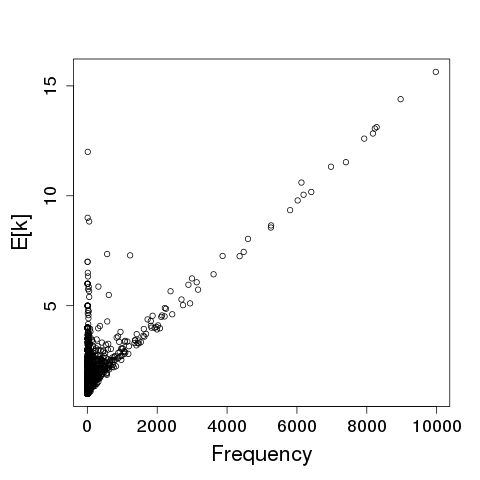
\includegraphics[width=0.47\textwidth]{graphs/ch4/tagalog-burstiness.png}
}
\subfloat[Adaptation\label{subfig:adaptation}]{
	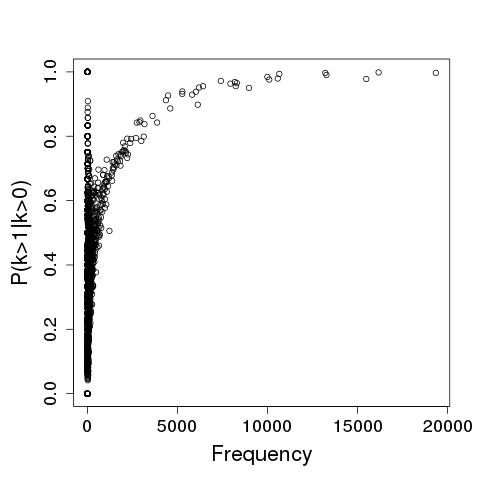
\includegraphics[width=0.47\textwidth]{graphs/ch4/tagalog-adaptation.png}
}
\caption[Burstiness and adaptation of Tagalog training vocabulary]{Burstiness and adaptation probability for Tagalog training vocabulary \label{fig:tagalogAdapt}}
\end{figure}

If we hold with the statement that ``Low frequency words tend to be rich in content, and vice-versa,"\cite{church1999}, then a significant number of content-rich keywords should exhibit this burstiness, and we can exploit this at search time.  While we do not claim any particular threshold defines ``content-rich", in the context of the Tagalog corpus, we observe that 26\% of all tokens and 25\% of low-frequency words ($f_w < 100$) have at least 50\% adaptation.  This is enough of a broad trend that we can indeed leverage this for improved search.

\subsection{Interpolation}

Now that we have a score interpolation model and a reasonable expectation of successful application, based on the observed strength of repetition in the data, we are faced with the choice for selecting an effective interpolation weight $\alpha$ (cf. Equation~\ref{eqn4:repetitionModel}).  How much should repetition matter?  Should we vary the interpolation weight by keyword or by document?  

Considering the adaptation probability, we can obtain an intuitive and effective interpolation weight directly from the training data.   The actual re-scoring depends only on scores local to $d$, so we need only a linear pass over the results for $d$ to obtain $\max\left[S_{kws}(h_{w,d})\right]$.  Not having to re-compute $\alpha$ avoids incurring additional computation at search time.  In addition, we showed in work published in 2014 that the effective interpolation weight also captured some inherent tendency towards repetition of each corpus. \cite{wintrode2014repetition}.

To illustrate, we consider two different methods for estimating $\alpha$.  First, we attempt to select different weights $\alpha_w$ on a per-keyword basis.  Alternatively we estimate a single $\widehat{\alpha}$ for each language (from the available training data).  We estimate each $\alpha$ based on the adaptation probability $P_{adapt}(w)$, but we find that the application is not trivial.  

Using the Tagalog Full LP (100 hour) training corpus and 10 hour development set, we empirically test the two approaches.  If we first compare estimates of $P_{adapt}$ for words that occur both in the training and development sets, we find, not surprisingly, that the difference between the two estimates is only consistent for high frequency words (cf. Figure~\ref{subfig:adaptTrainDev}).
\begin{align}
\alpha_w &= (1-e^{-\mathrm{DF}_w}) \cdot \widehat{P}_{adapt}(w)
\label{eqn4:alphaW} \\
\widehat{\alpha} &= \Avg_w\left[ \alpha_w \right] \label{eqn4:alphaHat}
\end{align}

Given this fact, when applying adaptation values learned from the training data to the search task, we discount our per-word $\alpha$ estimates based on the document frequency $DF_w$ (Equation~\ref{eqn4:alphaW}).  For a global interpolation, $\widehat{\alpha}$, we take the average over all the discounted per-word estimates.   Table~\ref{subfig:performance} shows the impact of these different choices for the interpolation weight in our keyword re-scoring formula (Equation~\ref{eqn4:repetitionModel}).  

\begin{figure}[t]
\subfloat[Difference in estimates of $P_{adapt}$ \label{subfig:adaptTrainDev}]{%
	\raisebox{-2cm}{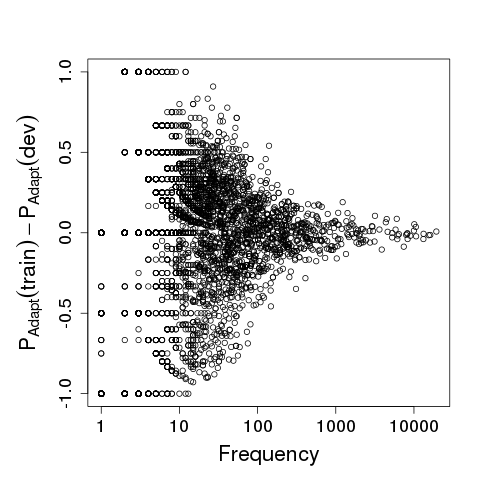
\includegraphics[width=0.4\textwidth]{graphs/ch4/train-eval-500.png}}\hfill
}
\subfloat[KWS Performance\label{subfig:performance}]{
\hfill
\begin{tabular}{lrr} \toprule
\bf Estimate& \bf TWV & \bf \bf $P(\mathrm{Miss})$ \\\midrule
None & 0.470 & 0.430 \\
$P_{adapt}(w)$ & 0.423 & 0.474 \\
$(1-e^{-\mathrm{DF}_w})P_{adapt}(w)$ &  0.477 & 0.415 \\
\textbf{$\widehat{\alpha}$ = 0.20} & \bf 0.483 & \bf 0.416 \\
\bottomrule \\[1ex]
& &  
\end{tabular}
%\vskip1cm
}
\caption[Estimating interpolation weights]{Estimating interpolation weights on Tagalog Full LP corpus\label{fig:tagalogInterp}}
\end{figure}

The global (per-language) interpolation weight clearly outperforms any other choice in terms of keyword accuracy (TWV).   The decrease in $P(Miss)$ is also an important result, because it indicates that our re-scoring does in fact boost repeated keywords above the detection threshold, increasing the number of correct keyword detections.  

We include our final estimate for $\widehat{\alpha}$ with the results for the Full LP (Table~\ref{fig4:FullLP}) and Limited LP condition (Table~\ref{fig4:LimitedLP}).  The relative values correspond to our expectations by language.  The lowest values (least repetition) occur for the Turkish data, a language known for its morphological complexity, hence word units are less likely to repeat.  The highest values occur for Cantonese and Vietnamese, which for the Babel program was transcribed with syllable-level word units.

\subsection{Experiments}
The complete procedure for each language in each condition (Limited or Full LP) is as follows.  We first estimate adaptation probabilities from the ASR training transcripts.  From these we take the weighted average as described, obtaining a single interpolation weight $\widehat{\alpha}$ for each language and training condition.   We train ASR acoustic and language models from the training corpus using the Kaldi speech recognition toolkit \cite{kaldi} following the default Babel training recipe which is described in detail by Chen et al.\cite{chen2013}

\begin{algorithm}
  \begin{algorithmic}[1]   
  \STATE \textbf{Estimate $\widehat{\alpha}$ on training corpus.}
  \STATE Train ASR Acoustic and Language Models
  \STATE Decode search audio corpus.
  \STATE Apply KWS algorithm
  \STATE \textbf{Re-score KWS results.}
  \end{algorithmic}
  \caption{Repetition-based term detection re-scoring}
  \label{alg4:repetition}
\end{algorithm}

We decode each development corpus with both Full and Limited LP models to generate ASR word lattices for the search task.  We then execute Kaldi's keyword search module which is an FST-based implementation of Saraclar and Sproat's lattice-based search speech search algorithm\cite{saraclar2004}.  Lastly, we re-score the search output by interpolating the top term detection score for a document with subsequent hits according to Equation~\ref{eqn4:repetitionModel} using the $\widehat{\alpha}$ estimated for the corresponding training condition.  We outline these steps in Algorithm~\ref{alg4:repetition}, re-iterating that our contributions, steps 1 and 5, can be carried out regardless of the ASR/KWS specifics of steps 2-4.

\begin{table}
\centering
\begin{tabular}{l|l|r|r} \toprule
\bf Language & \bf $\widehat{\alpha}$ & \bf TWV (\%$\pm$) & \bf $P(\mathrm{Miss})$ (\%$\pm$) \\\midrule
\multicolumn{4}{c}{Full LP setting} \\\midrule
Tagalog & 0.20 & \textbf{0.523} $\,$ (+1.1) & 0.396 $\,$ (-1.9)\\
Cantonese & 0.23 & \textbf{0.418 }$\,$ (+1.3) & 0.458 $\,$ (-1.9) \\
Pashto & 0.19 & \textbf{0.419} $\,$ (+1.1) & 0.453 $\,$ (-1.6) \\
Turkish & 0.14 & \textbf{0.466} $\,$ (+0.8) & 0.430 $\,$ (-1.3) \\
Vietnamese & 0.30 & \textbf{0.420} $\,$ (+0.7) & 0.445 $\,$ (-1.0) \\
%\midrule
%\textit{English (Dev06)} & 0.20 & \bf 0.670 $\,$ (+0.3) & 0.240 $\,$ (-0.4) \\
\bottomrule
\end{tabular}
\caption[Word-repetition re-scored results]{Word-repetition re-scored results for Full LP term detection corpora, improvement over baseline system denoted as percentage change. 
\label{fig4:FullLP} }
\end{table}


The overall improvements of our re-scoring algorithms are given in Table~\ref{fig4:FullLP} (Full LP) and Table~\ref{fig4:LimitedLP}.  In both Full LP and Limited LP settings, using only keyword repetition information, we observe improved KWS accuracy in terms of TWV between 0.7 and 1.3\% absolute.   Just as importantly, given TWV can be improved by either reducing false alarms or reducing misses, we decrease the miss probability in all but one condition (the exception being Vietnamese Limited LP).  

The reduction in $P(Miss)$ indicates that the proposed re-scoring approach does in fact do what we intend - raise the scores of repeated keywords above the system threshold.  Keywords that otherwise were unlikely under either the ASR acoustic or language model are indeed boosted because they occur elsewhere in the document.


\begin{table}
\centering
\begin{tabular}{l|l|r|r} \toprule
\bf Language & \bf $\widehat{\alpha}$ & \bf TWV (\%$\pm$) & \bf $P(\mathrm{Miss})$ (\%$\pm$) \\\midrule
\multicolumn{4}{c}{Limited LP setting} \\\midrule
Tagalog & 0.22 & \textbf{ 0.228} $\,$ (+0.9) & 0.692 $\,\,\,$ (-1.7)\\
Cantonese & 0.26 & \textbf{0.205} $\,$ (+1.0) & 0.684 $\,\,\,$ (-1.3) \\
Pashto & 0.21 & \textbf{0.206 }$\,$ (+0.9) & 0.682 $\,\,\,$ (-0.9) \\
Turkish & 0.16 & \textbf{0.202} $\,$ (+1.1) & 0.700 $\,\,\,$ (-0.8) \\
Vietnamese & 0.34 & \textbf{0.227} $\,$ (+1.0) & 0.646 $\,$ (+0.4) \\
\bottomrule
\end{tabular}
\caption[Word-repetition re-scored results]{Word-repetition re-scored results for Limited LP term detection corpora, improvement over baseline system denoted as percentage change. 
\label{fig4:LimitedLP} }
\end{table}


\section{Language Model Adaptation}

Whereas for the keyword repetition model we treat ASR/KWS systems as a black box, we now consider the effect of adding topic context directly to the ASR system's language model explicitly.  By representing broad and local context as word N-gram probabilities that are re-computed on a document by document or utterance by utterance basis, we can use the adaptation methods described in Section~\ref{sec:scores} to augment the system's baseline N-gram model. 

Given the augmented language model can be used either to \textit{re-score} existing lattice output or to \textit{re-decode} the audio to generate new lattices.  We can show that adding topic context to the language model improves search accuracy in both cases, and in particular, combining both types of context (local and broad) improves accuracy of either approach individually.

Re-scoring corresponds to the re-computing the language model scores on an existing lattice $\mathcal{L}$ (cf. Eqns.~\ref{eqn:latrescore1},\ref{eqn:latrescore2}).  
The structure of $\mathcal{L}$ and thus the words it represents are unchanged, but ideally the correct words in a more accurate model would re-score higher than incorrect words.  Re-decoding, by contrast, constructs an entirely new lattice $\mathcal{L}^{\prime}$, by modifying the decoding graph $HCLG$.
\begin{equation}
\mathcal{L}^{\prime} \approx S \equiv U \circ (H\circ C\circ L\circ G_{adapted})
\end{equation}
As lattice-generation involves pruning the search space, low likelihood word hypotheses are removed from the final lattice. Changing the language model at this stage can cause a different set of words to appear in the lattice.  By measuring lattice keyword recall, we can also show that by decoding with topic-augmented language models, more correct keywords survive the pruning process, which contributes to a larger search accuracy improvement.


\subsection{Latent Topic Language Models}
\label{sec:ltlm}
We represent the broad topic context of a document using a standard LDA topic model. In LDA and similar latent topic models, words and documents are modeled as arising from a document-specific mixture of $\mathcal{T}$ topics.  A topic in this framework is a multinomial distribution over the corpus vocabulary - a unigram language model.  A document's topic context is encoded by the inferred topic mixture for that document, $\theta^{(d)}$.  We will look at parameter estimation and inference in detail in the next chapter.  We obtain estimates for $\phi$ and $\theta^{(d)}$ then use the latter as a set of mixture weights to compute a \textit{document-specific} unigram language model $P_{T}(w|\theta^{(d)})$ (cf. Equation~\ref{eqn4:unigramMix}).  This document-specific model can then be used to adapted the original LM as we described previously.
\begin{align}
P_T(w|\theta^{(d)}) &= \sum_{t=1}^{\mathcal{T}} {\theta^{(d)}_t\cdot \phi^{(t)}_w} \label{eqn4:unigramMix} 
%\\
%P_Ld(w) &= \lambda P_L(w) + (1-\lambda) P_T(w|d) \label{eqn4:interp1}
\end{align}

%The LDA generative process is presented as Algorithm~\ref{alg4:LDA}.  
%\begin{algorithm}
%  \begin{algorithmic}[]                                    
%  \FORALL {$t\in \mathcal{T}$}                             
%          \PRINT{$\phi^{(t)}\sim\mbox{Dirichlet}(\beta)$}  
%  \ENDFOR                                                  
%
%  \FORALL{$d\in\mathcal{D}$}
%          \PRINT{$\theta^{(d)}\sim\mbox{Dirichlet}(\alpha)$}
%         \FOR{ $w_{d,i}, 1 \le i \le |d|$}
%				\PRINT{$z_{d,i}\sim\theta^{(d)}$} 
%                \PRINT{$w_{d,i}\sim\phi^{(t=z_{d,i})}$}
%          \ENDFOR
%   \ENDFOR
%%   \vskip0.25cm
%  \end{algorithmic} 
%  \caption{\label{alg4:LDA} LDA generative process}
%\end{algorithm}

For each language in our experiments we learn a latent topic (LDA) model from the training corpus transcripts.  We use the Gibbs sampling approach as implemented in the Mallet toolkit \cite{mallet}, with minor modifications in order to allow operations on soft counts (i.e. lattice expected counts). Model estimation yields $\mathcal{T}$ topics, prior probabilities $\alpha^{(t)}$ for each topic, and the symmetric Dirichlet hyperparameter $\beta$ for the unigram distributions \cite{steyvers2007}.  The $\theta^{(d)}$ for the training data are computed, but not used for our task. 

In order to compute $\theta^{(d)}$ for the documents in the search corpus we apply the Gibbs sampler, seeded with the learned model parameters, to expected word counts extracted from lattices generated by the baseline ASR system.  Our baseline system for the experiments in this section and in Chapter 7 deep neural net (DNN) acoustic models and a 3-gram backoff language model, described in detail in \cite{wintrode2014slta} and elsewhere.    Given $\theta^{(d)}$ for the test lattices and $\phi^{(t)}$ from the training transcripts, we can compute the document-specific unigram models for adaptation.  We also conducted oracle experiments using the true test transcripts to infer $\theta^{(d)}$ mixture weights on the test data, and the term detection results were identical to the fair results presented here.

We apply our topic-adapted language models to ASR/KWS systems built under the Limited LP setting in Tagalog, Vietnamese, Zulu, and Tamil.  We test the topic-adapted models for both re-scoring and re-decoding the development data.  We adapted the baseline model using linear interpolation (cf. Eqn.~\ref{eqn4:linear}) with interpolation weight $\lambda$. We showed in \cite{wintrode2014slta} that we can select the $\lambda$ that minimizes perplexity on the first pass one-best output, and that approach is reflected in the results in Table~\ref{fig4:topicLM}.

%We incorporate the two language models, which we denote $P_T$ and $P_L$ respectively using a linear interpolation of the unigram probabilities (cf. Equation~\ref{eqn4:interp1}).  This gives us a distinct topic-specific language model for each document.  This approach does require selecting an interpolation weight $\lambda$.  


\begin{table}
\centering
   \begin{tabular}{l|l|rrr} \toprule
   \bf Language & \bf Metric & \bf N-Gram & \bf LDA(R) & \bf LDA(D) \\ \midrule
Tagalog& WER & 60.8 & 61.6 & 61.6  \\
        & TWV & 0.244 & \textbf{0.247} & \textbf{0.254}\\
        & L. Recall & 0.778 & 0.778 & \textbf{0.792}\\ \midrule
Vietnamese &   WER & 62.0 & 61.9 & 62.1  \\
        & TWV & 0.254 & \textbf{0.257} & \textbf{0.269}\\
        & L. Recall & 0.555 & 0.555 & \textbf{0.567}\\ \midrule
Zulu&   WER & 67.8 & 68.2 & 68.1  \\
        & TWV & 0.270 & \textbf{0.278} & \textbf{0.283}\\
        & L. Recall & 0.718 & 0.718 & \textbf{0.739}\\ \midrule
Tamil&   WER & 76.0 & 76.1 & 76.2  \\
        & TWV & 0.216 & \textbf{0.226} & \textbf{0.237}\\
        & L. Recall & 0.573 & 0.573 & \textbf{0.622}\\ \bottomrule
        \end{tabular}
\caption[Re-scoring and re-decoding with topic-augmented LMs]{Recognition and retrieval performance re-scoring and re-decoding with topic-augmented LMs  \label{fig4:topicLM}}
\end{table}


The results in Table~\ref{fig4:topicLM} illustrate the importance of focusing on retrieval performance and not just word error rate (WER).  The topic-adapted language models in most cases increase WER, and if that were our only metric, we would perhaps disregard the technique.  However, re-scoring with topic information increases retrieval accuracy by 0.3 to 1.0\% absolute and re-decoding improves keyword retrieval by 1.0 to 2.1\%.  

Additionally, applying topic-augmented models at decoding time increases the overall recall of keyword occurrences (Lattice Recall) from 1.2 to 4.9\%.  We can conclude that the topic context, which in cases where the keywords were not in the baseline lattices, can in fact boost the probabilities for topically related words such that they survive the pruning process and can be retrieved by the KWS system.

% reference to whitelisting?

\subsection{Cache-based Language Models}

We incorporate local context by implementing a cache-augmented language model. The approach we adopt here and in \cite{wintrode2014slta} is based off of the work from Jelinek \cite{jelinek1991} and Kuhn \cite{kuhn1990} where we leverage the assumption that a local word or N-gram frequency estimate may be more reliable than the global frequency. Here we adapt the base language model via the \textit{count merging} method of model interpolation.  For a contrastive system, we implemented the discriminative trigger model from \cite{singh2007trigger}.    

We define the local context for a particular utterance specifically as the expected lattice-counts for N-grams from \textit{all other utterances in the document}.  We also experimented with a exponentially decaying cache (cf. \cite{clarkson1997}) that favors adjacent utterances but found no difference in performance.  For each utterance we compute an adapted language model by adding the expected lattice counts for N-grams in the local context to the original training frequencies (count-merging).  In our implementation of the Singh-Collins trigger models we use the same context in computing the trigger activation.

%\begin{equation}
%f_{adapted}(w_{[i,i+N-1]}) =f_{train}(w_{[i,i+N-1]}) + \lfloor{\beta\cdot %f_{doc}(w_{[i,i+N-1]})}\rfloor  \label{cacheq}
%\end{equation}

The interpolation parameter $\beta$ for the count-merging approach (cf. Eqn.~\ref{eqn:countmerge}) can be interpreted as a scaling factor on the local counts.   We experimented with a coarse set of scaling factors, $\beta=[1,5,10,20]$, but found empirically that no additional gain was found beyond $\beta=10$.  Re-estimating backoff language models on an utterance by utterance basis using the SRI Language Modeling toolkit\cite{srilm} (SRILM), we required the use of the $floor$ function on the fractional expected lattice N-gram counts.  This also had the effect, with $\beta=10$ of pruning any counts with posterior probability of less than 0.1. 

For the contrastive trigger model, we trained the perceptron models as described in \cite{roark2004discriminative}, by decoding the training corpus and generating 100-best hypotheses for each training utterance.  Each perceptron model on which we report was trained with 2 iterations over the data as in the previous work.  For the test data we instantiated the discriminative model directly as the FST $\mathcal{D}$ and performed the composition with the output lattice.

As with the topic-specific language models, we re-score each output lattice and apply the Kaldi lattice keyword search to the re-scored lattices.  Unlike the topic-specific models, the cache-augmented language models reduce WER on the Babel development data and increases term detection accuracy from 0.2\% to 1.6\% absolute (cf. Table~\ref{fig4:cachelms}).  The discriminative trigger model performs noticeably worse, the reported results arising from unigram-only trigger features, which outperformed any other feature combination from \cite{singh2007trigger} when applied to the Babel data.  However we would point out that the WER of the Babel systems are at least twice that of the English systems used to train the trigger models in \cite{singh2007trigger} and the resulting lattice scores not well calibrated posterior probabilities, which would more negatively impact the TWV score.

\begin{table}
\centering
   \begin{tabular}{l|l|rrr} \toprule
   \bf Language & \bf Metric & \bf N-gram & \bf Trigger(R) & \bf Cache(R) \\ \midrule
Tagalog& WER & 60.8 & 61.7 & \textbf{60.3} \\
        & TWV & 0.244 & 0.161 & \textbf{0.260} \\ \midrule
Vietnamese &   WER & 62.0 & 63.7 & \textbf{61.5}  \\
        & TWV & 0.254 & 0.190 & \textbf{0.256} \\ \midrule
Zulu&   WER & 67.8 & 69.2 & \textbf{67.5} \\
        & TWV & 0.270 & 0.192 & \textbf{0.276} \\ \midrule
Tamil&   WER & 76.0 & 76.9 &  \textbf{75.5}  \\
        & TWV & 0.216 & 0.138 &\textbf{0.229} \\ \bottomrule
        \end{tabular}
\caption[Re-scoring with cache-augmented LMs]{Recognition and retrieval performance re-scoring with cache-augmented LMs  \label{fig4:cachelms}}
\end{table}

\section{Conclusion}

Lastly, we look at the broad and local contexts in terms of complementary information.  In \cite{wintrode2014slta} we showed how we could apply the cache re-scoring after decoding with the topic-augmented language models.  This result, for the Babel corpora is described for both recognition  (WER) and retrieval (TWV) in Table~\ref{fig4:cascade}.  The cascaded result strongly suggests that the two types of topic context, while related, provide complementary information for the retrieval task.

\begin{table}
\centering
   \begin{tabular}{l|l|rrrr} \toprule
   \textbf{Language} & \textbf{Metric} & \textbf{N-gram} & \textbf{Cache(R)} & \textbf{LDA(D)} & \textbf{LDA+Cache} \\ \midrule
Tagalog & WER & 60.8 & 60.3 & 61.6 & \textbf{59.7} \\
        & TWV & 0.244 & 0.260 & 0.254 & \textbf{0.267} \\ \midrule
Vietnamese &   WER & 62.0 & \textbf{61.5} & 62.1 & 61.8 \\
        & TWV & 0.254 & 0.256 & 0.269 & \textbf{0.271}\\ \midrule
Zulu&   WER & 67.8 & 67.5 & 68.1 & \textbf{67.4} \\
        & TWV & 0.270 & 0.276 & 0.283 & \textbf{0.289} \\ \midrule
Tamil&   WER & 76.0 & 75.5 & 76.2 & \textbf{75.4}\\
        & TWV & 0.216 & 0.229 & 0.237 & \textbf{0.240} \\ \bottomrule
        \end{tabular}
\caption[Combined topic and cache-augmented LMs]{Recognition and retrieval performance with topic-augmented decoding followed by cache re-scoring.  \label{fig4:cascade}}
\end{table}

\begin{figure}
\begin{center}
\subfloat[Tagalog\label{subfig4:tagalog}]{%
    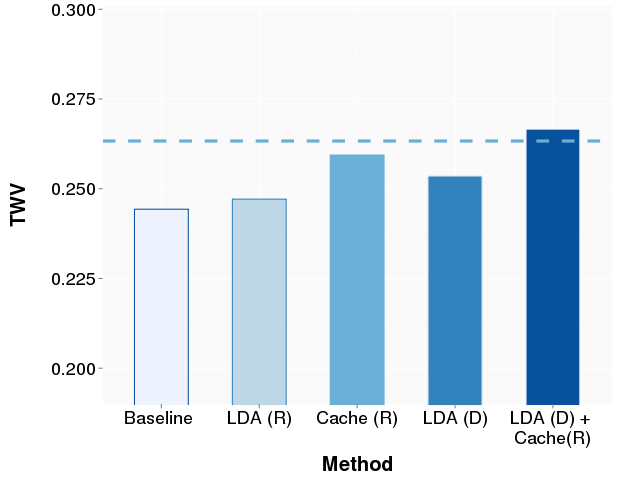
\includegraphics[width=0.47\textwidth]{graphs/ch4/Tagalog-rescore.png}
}
\subfloat[Vietnamese\label{subfig4:vietnamese}]{
	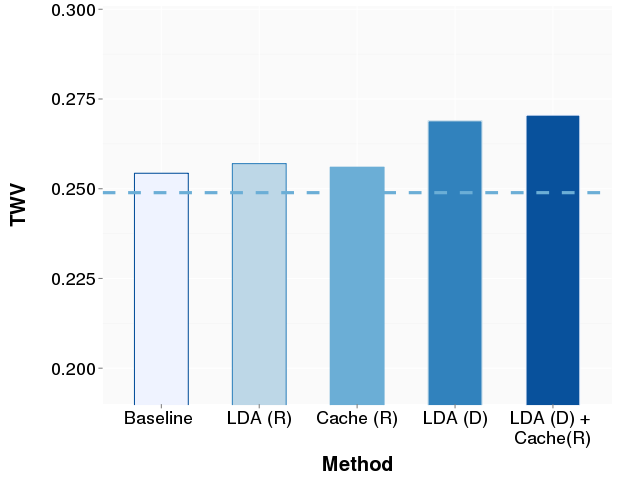
\includegraphics[width=0.47\textwidth]{graphs/ch4/Vietnamese-rescore.png}
}\\
\subfloat[Zulu\label{subfig4:zulu}]{%
    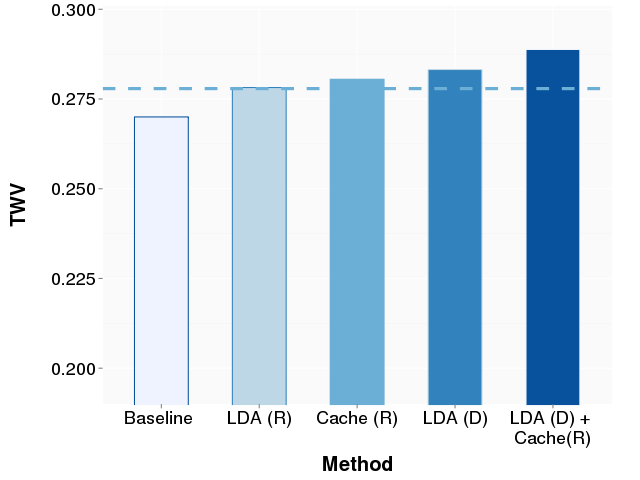
\includegraphics[width=0.47\textwidth]{graphs/ch4/Zulu-rescore.png}
}
\subfloat[Tamil\label{subfig4:tamil}]{
	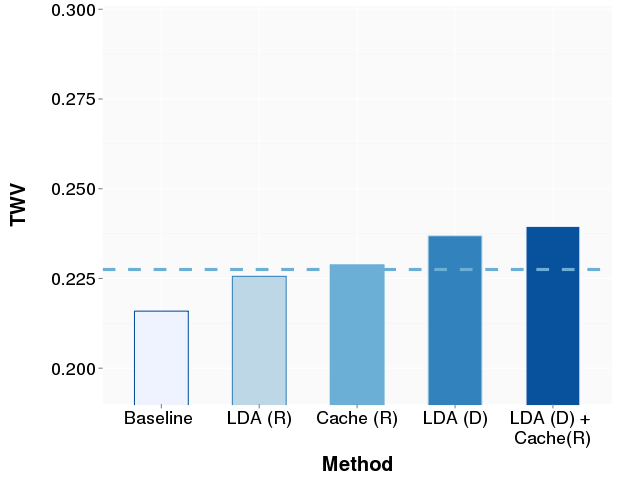
\includegraphics[width=0.47\textwidth]{graphs/ch4/Tamil-rescore.png}
}
\end{center}
\caption[Term detection performance with topic-augmented adapted LMs]{Term detection performance when adapting ASR language models.  Dashed line indicates ad-hoc repetition performance.\label{fig4:fullLMResults}}
\end{figure}

We illustrate the overall performance impact of incorporating topic context directly into the ASR language model in Figure~\ref{fig4:fullLMResults}.  The overall conclusion is as we hoped, that both broad context, implemented as topic mixture models, and local context, implemented as cached N-grams, when added to the language model, improve keyword retrieval performance.     

In general, across all 4 languages re-decoding with the topic-augmented models, denoted \textbf{LDA(D)}, outperforms simply re-scoring existing lattices, denoted \textbf{LDA(R)}.  The relative performance of local context, \textbf{Cache(R)} versus the LDA models depended on the language.  In Zulu and Tamil, the cache re-scoring outperformed the LDA re-scoring, but not re-decoding.   In Tagalog, the cache re-scoring outperformed both \textbf{LDA(R)} and \textbf{LDA(D)}.  In Vietnamese, the cached models only slightly outscored the baseline. 

For comparison we include the performance of the non-LM repetition re-scoring algorithm described in the first half of the chapter, represented as the dashed line in Figure~\ref{fig4:fullLMResults}.  As we might expect, this method tracks with the cache results, performing best on the Tagalog corpus, where the cache-adapted LM also out-performed other methods, and underperforms on Vietnamese, just as the \textbf{Cache(R)} approach.  % interpolation weight

The final conclusion we can draw from our experiments is that the combination of \textbf{LDA(D)} and \textbf{Cache(R)} in a simple cascade outperforms each method individually, in all 4 languages.  This result leads us to assert that the two types of topic context, while related, are complementary, and in the remaining chapters we will consider a joint model of the two phenomena, with an eye towards retrieval performance.

